\documentclass[letterpaper,12pt,twoside,]{pinp}

%% Some pieces required from the pandoc template
\providecommand{\tightlist}{%
  \setlength{\itemsep}{0pt}\setlength{\parskip}{0pt}}

% Use the lineno option to display guide line numbers if required.
% Note that the use of elements such as single-column equations
% may affect the guide line number alignment.

\usepackage[T1]{fontenc}
\usepackage[utf8]{inputenc}

% pinp change: the geometry package layout settings need to be set here, not in pinp.cls
\geometry{layoutsize={0.95588\paperwidth,0.98864\paperheight},%
  layouthoffset=0.02206\paperwidth, layoutvoffset=0.00568\paperheight}

\definecolor{pinpblue}{HTML}{185FAF}  % imagecolorpicker on blue for new R logo
\definecolor{pnasbluetext}{RGB}{101,0,0} %


\usepackage{wrapfig,subcaption,array,tabularx,multirow,caption} \usepackage[utf8]{inputenc}

\title{QBUS2820 Assignment2}

\author[]{}


\setcounter{secnumdepth}{0}

% Please give the surname of the lead author for the running footer
\leadauthor{}

% Keywords are not mandatory, but authors are strongly encouraged to provide them. If provided, please include two to five keywords, separated by the pipe symbol, e.g:
 

\begin{abstract}

\end{abstract}

\dates{This version was compiled on \today} 

% initially we use doi so keep for backwards compatibility
% new name is doi_footer

\pinpfootercontents{QBUS2820 Assignment 1}

\begin{document}

% Optional adjustment to line up main text (after abstract) of first page with line numbers, when using both lineno and twocolumn options.
% You should only change this length when you've finalised the article contents.
\verticaladjustment{-2pt}

\maketitle
\thispagestyle{firststyle}
\ifthenelse{\boolean{shortarticle}}{\ifthenelse{\boolean{singlecolumn}}{\abscontentformatted}{\abscontent}}{}

% If your first paragraph (i.e. with the \dropcap) contains a list environment (quote, quotation, theorem, definition, enumerate, itemize...), the line after the list may have some extra indentation. If this is the case, add \parshape=0 to the end of the list environment.


\hypertarget{introduction}{%
\section{Introduction}\label{introduction}}

In a traditional manner, sale prices of houses were predicted by
comparing sale prices and costs in the real estate market. There was no
general standard to estimate the value of houses. Machine learning
techniques therefore play an important role to help establishing models
for sale prices of house predictions. As mentioned by Calhoun, the
availability of a house price prediction model helps fill up an
essential information gap and improve the efficiency of the real estate
market (Calhoun, 2003).

This project aims to develop predictive models for sale prices of house
with machine learning techniques. With the sale price which is a
numerical variable being the response of predictive models, six models
are developed and validated.

By comparing the root mean squared errors of predictions, the lasso
regression model and random forest model are found to have the best
predictive performance for the housing data, compared to elastic net,
ridge regression, k-nearest neighbour regression and stepwise
regressioin with forward selection.

\hypertarget{data-processing-and-exploratory-data-analysis}{%
\section{Data processing and exploratory data
analysis}\label{data-processing-and-exploratory-data-analysis}}

There are 36 numeric variables and 43 categorical variables in the
housing data

\hypertarget{feature-engineering}{%
\section{Feature engineering}\label{feature-engineering}}

\begin{wrapfigure}{r}{0.5\textwidth}
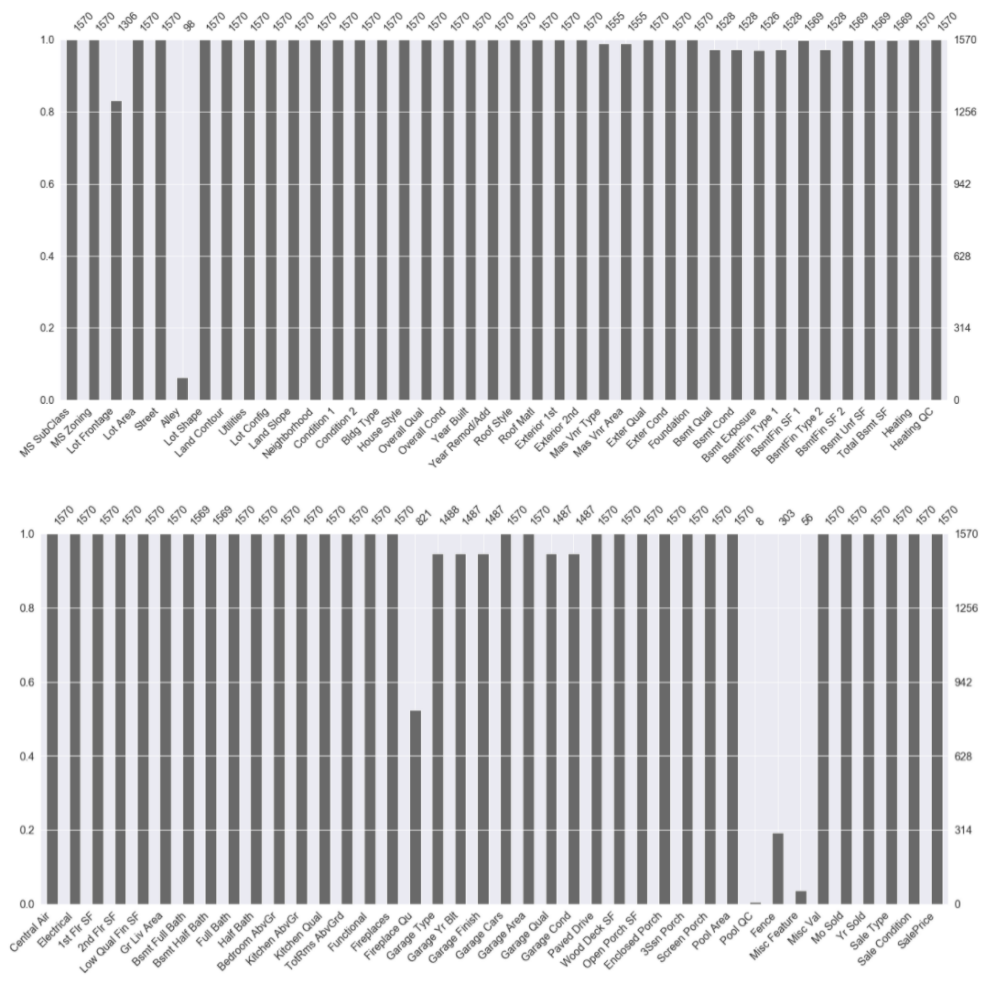
\includegraphics[width=1\linewidth]{miss_plot.png}
\centering
\caption{Visualizing missingness of housing data.}
\label{fig:miss}
\end{wrapfigure}

As shown in Figure \ref{fig:miss}, there are huge amounts of missing
values in several columns: `Alley', `Fireplace Qu', `Pool QC', `Fence',
`Misc Feature'. By calculating the number of null values, these 5
columns are found to have more than 40\% missing values within each
column. With this issue, such variables are uninformative to ba a
feature of predictive models as too few observations are provided.
Removing all rows with missing values can lead to significant loss of
data while imputation is not appropriate for such largely incomplete
columns. Therefore, `Alley', `Pool QC', `Fence', `Misc Feature' are
abandoned.

Besides, there are 19 columns containing missing value but the
percentages of missing values are less than 20\%. This can be dealed
with by imputation. The missing values are imputed by using the most
frequent value of each columns.

To deal with outliers of numeric features, standardisation is performed
by subtracting the mean, followed by dividing the standard deviation of
the corresponding columns.

After feature engineering, there are 74 informative features, with 36
features being numerical and 38 features being categorical. There are
1570 in the training set while 1210 observations remain in the testing
set. In order to involve categorical features in regression models,
dummy variables are created for each categorical feature.

\hypertarget{methodology}{%
\section{Methodology}\label{methodology}}

\hypertarget{validation-set}{%
\section{Validation set}\label{validation-set}}

%\showmatmethods


\renewcommand\refname{Conclusion}
\bibliography{pinp}
\bibliographystyle{jss}



\end{document}

